\documentclass[11pt]{article}

\usepackage{changepage}
\usepackage{graphicx}
\usepackage{amssymb} %math symbols
\usepackage{mathtools} %more math stuff
\usepackage{amsthm} %theorems, proofs and lemmas
\usepackage{optidef} %fast optimization problem notation
\usepackage{biblatex} %Imports biblatex package
\addbibresource{papers.bib} %Import the bibliography file

\usepackage{minted} % code highlighting

%% declaring abs so that it works nicely
\DeclarePairedDelimiter\abs{\lvert}{\rvert}%
\DeclarePairedDelimiter\norm{\lVert}{\rVert}%

\title{MICRO-453 - Boxfish robotics practical}
\author{Gabriel Vallat, Lucas Bost, Titouan Renard}

\begin{document}

\maketitle
\tableofcontents
\section{Introduction and presentation of the hardware}

\begin{figure}[h!]
    \centering
    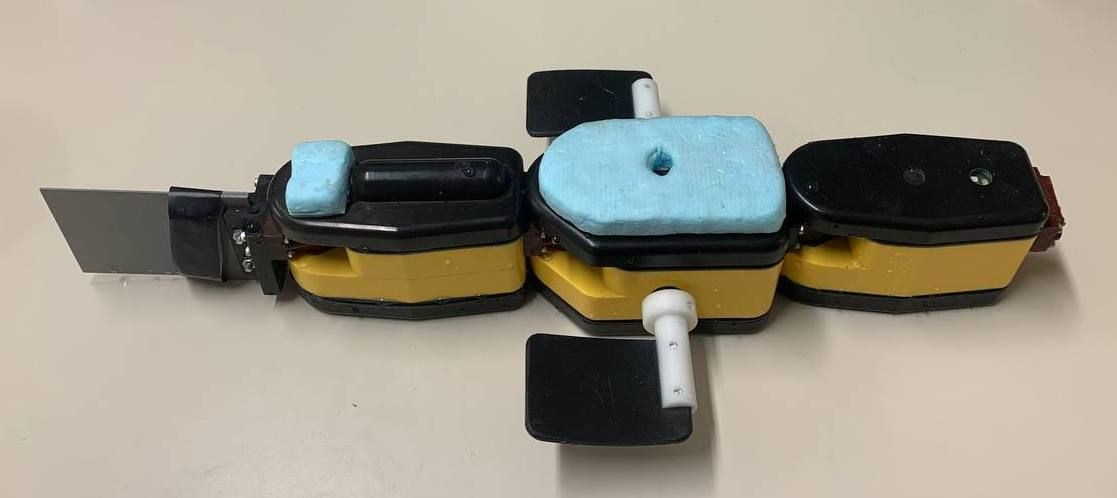
\includegraphics[width=0.8\textwidth]{figures/side.jpg}
    \caption{Sideview of the boxfish robot.}
    \label{boxfish}
\end{figure}

This report presents results from a practical session from the MICRO-453 course. It discusses the implementation of a simple control algorithm for a \textit{boxfish} bioinspired robot built out of \textit{salamadra robotica II} modules \cite{salamadra_robotica_2}. The robot is build of $3$ modules and has $4$ actuators. 

\section{On-board and off-board software}


\subsection{Compiling and flashing the robot's microcontroller}

The first program is changing the color of the LED in an infinite loop. It uses the function \texttt{set\_rgb(uint8\_t r, uint8\_t g, uint8\_t b)}, where r, g and b are the intensities of color red, green and blue respectively (between 0 and 127). In the program the value of one color channel is changed every 10 ms (the delay is induced with the function \texttt{pause()}). %The LED first goes from extinct to red, then from red to yellow, from yellow to white, from white to cyan, from cyan to blue and from blue to extinct, and then it repeats this pattern. When we compile and run the program, the result is what we expected. 
To make the LED blink in green at 1 Hz, we change the part of the code in the infinite loop. We first light the LED in green setting the green channel to its max and red and blue to their min (\texttt{set\_rgb(0,127,0)}). % to set only the green channel. Then we write pause(HALF\_SEC) so that the light emits light during 0.5 second. And after we extinct the LED with \texttt{set\_rgb(0,0,0)} and the LED stays extinct during 0.5 second.
\\
\\
For the part with the registers and the radio communication, to predict the display of the program we have to predict the display of the function \texttt{read\_registers()} in ex2.cc. In \texttt{read\_registers()} there are some calls to the function \texttt{get\_reg\_b}, which consists of a read operation in the 8 bits registers. The first call is \texttt{regs.get\_reg\_b(6)}, so it will be a reading access in the 8-bits register of address 6. In the program main.c, in the register callback function it corresponds to a ROP\_READ\_8 operation. In the switch, in the case \texttt{ROP\_READ\_8} at the address 6, we see that the value of the counter is assigned in radio\_data${\rightarrow}$byte, which is the value that is retrieved by the function \texttt{get\_reg\_b}. The value of the counter at the beginning is 0, so the value retrieved will be 0. In this case the counter is also set to 0 so here its value is unchanged. The second call is \texttt{regs.get\_reg\_b(21)} which corresponds in the switch to an operation \texttt{ROP\_READ\_8} at address 21. In this case a constant vaue of \texttt{0x42} is assigned in \texttt{radio\_data}${\rightarrow}$\texttt{byte} and the counter is incremented (i.e. counter = 1). The third call is once again \texttt{regs.get\_reg\_b(21)}, so the value that will be retrieved by the funciton is \texttt{0x42} and the counter will be incremented again (i.e. counter = 2). The fourth call is \texttt{regs.get\_reg\_b(6)}, so the value of the counter (counter = 2) will be retrieved and the counter is set back to 0. The last call is \texttt{regs.get\_reg\_b(6)}, so the value that will be retrieved is 0.
Then there is a call of \texttt{display\_multibyte\_register(reg, 2)}. In this function, the program tries to read the content of the multibyte register of address 2 (\texttt{get\_reg\_mb()}). It displays the size of the buffer that is read (content of radio\_data${\rightarrow}$multibyte.size) and the content of the buffer (\texttt{radio\_data${\rightarrow}$multibyte.data[]}). In main.c, the function \texttt{get\_reg\_mb} at address 2 corresponds to the operation \texttt{ROP\_READ\_MB} at the address 2. In this case the variable \texttt{last\_mb\_size} is stored into \texttt{radio\_data}${\rightarrow}$\texttt{multibyte.size} and the variable \texttt{mb\_buffer[]} is stored into \texttt{radio\_data}${\rightarrow}$\texttt{multibyte.data[]}. At the beginning, \texttt{last\_mb\_size} is equal to 0 and there is nothing in \texttt{mb\_buffer} so the display will just be the size of the buffer which is 0. Then a buffer is created and the resulting buffer is: \texttt{[100,101,102,103,104,105,106,107]}. There is a call of \texttt{regs.set\_reg\_mb(2, buffer, sizeof(buffer)}, which corresponds to a writing operation in the multibyte of address 2. In \texttt{main.c} this is an operation \texttt{ROP\_WRITE\_MBWe} at address 2. In this case the content of \textttt{radio\_data}${\rightarrow}$\texttt{multibyte.size} is assigned to the variable \texttt{last\_mb\_size} and the content of \texttt{radio\_data}${\rightarrow}$\texttt{multibyte.data[]} is assigned into \texttt{mb\_buffer}, but every value of the buffer is incremented by 4. The value of \texttt{last\_mb\_size} is thus 8 and the content of the content of \texttt{mb\_buffer} is [104, 105, 106, 107, 108, 109, 110, 111]. Then there is a call of function \texttt{display\_multibyte\_register(regs, 2)}. In main.c it corresponds to an operation \texttt{ROP\_READ\_MB} at address 2. In this case the value of \texttt{last\_mb\_size} (it's equal to 8) is assigned in \texttt{radio\_data}${\rightarrow}$\texttt{multibyte.size} and the content of \texttt{mb\_buffer[]} is assigned in \texttt{radio\_data}${\rightarrow}$\texttt{multibyte.data[]} ([104,105,106,107,108,109,110,111]) and the display will be the size of the buffer and the buffer itself. Then there's a call set\_reg\_b(2, 11) which corresponds to a \texttt{ROP\_WRITE\_8} operation at address 2. In this case the first value of \texttt{mb\_buffer} is replaced by the value stored in \texttt{radio\_data}${\rightarrow}$\texttt{byte} which is equal to 11. For the call \texttt{set\_reg\_b(3, 22)} it's quite the same but the address is 3 and this is the second element of \texttt{mb\_buffer} that is replaced by the value contained in radio\_data${\rightarrow}$byte which is equal to 22. Then comes another call of \texttt{display\_multibyte\_register} so the display will be the size of the buffer (which hasn't changed) and \texttt{mb\_buffer} ([11,22,106,107,108,109,110,111]). Then we have a call of function \texttt{regs.set\_reg\_w(7,2121)} which corresponds in main.c to an operation \texttt{ROP\_WRITE\_16} (writing in 16 bits registers) at address 7. In the switch, in this case the value of a variable \texttt{datavar} is multiplied by 3 and incremented by the value stored in \texttt{radio\_data}${\rightarrow}$\texttt{word}. At the beginning the value of \texttt{datavar} is 0 and here the value contained in \texttt{radio\_data}${\rightarrow}$\texttt{word} is 2121 so the new value of \texttt{datavar} will be: ${3\times0 + 2121 = 2121}$. Then with \texttt{regs.get\_reg\_dw(2)} the program performs a reading operation in 32-bits registers. In the switch this corresponds to an operation \texttt{ROP\_READ\_32} at address 2. In this case the value of \texttt{datavar} is assigned in \texttt{radio\_data}${\rightarrow}$\texttt{word} and the display is the value of \texttt{datavar}. Then with the call \texttt{regs.set\_reg\_w(7,1765)} the new value of \texttt{datavar} is ${3\times2121 + 1765 = 8128}$. And finally with the last call of \texttt{regs.get\_reg\_dw(2)}, the new value of \texttt{datavar} is displayed. So the predicted display is:


\begin{minted}{c}
get_reg_b(6) = 0
get_reg_b(21) = 66
get_reg_b(21) = 66
get_reg_b(6) = 2
get_reg_b(6) = 0
get_reg_mb(2) = 0 // bytes:
get_reg_mb(2) = 8 // bytes: 104, 105, 106, 107, 108, 109, 110, 111
get_reg_mb(2) = 8 // bytes: 11, 22, 106, 107, 108, 109, 110, 111
get_reg_dw(2) = 2121
get_reg_dw(2) = 8128
\end{minted}

When we compile the program and run it, the result is the same as expected.

\subsection{Internal communication between the robot's modules}

In this part, in the main.c a body module (motor) is initialized. It uses the function of the CAN to store in a variable pos (signed integer on 8 bits) the value that is contained in the CAN register of address \texttt{MREG\_POSITION} in the module of address \texttt{MOTOR\_ADDR} with the function \texttt{bus\_get(MOTOR\_ADDR, MREG\_POSITION)}. This value is just the position of the actuator of address \texttt{MOTOR\_ADDR}. It uses the function \texttt{set\_rgb} to lights a LED in different color ranges depending on the sign of the position and the value of the position itself. When we compile the program and run it, we observe that the color of the LED is changing when we move the actuator by hand.
\\
\\
In order to get back continuously the position of the 4 actuators of the boxfish, we need to do several things. We first need to create a c++ file to be able to read values that are sent by radio from the robot to the computer. This program is quite similar to ex2.cc. We keep the function display\_multibyte\_register and only modify it a little bit so that the display is "Body dof, limb first dof, limb second dof and limb third dof positions are respectively: pos1, pos2, pos3, pos4". In the main function, we just add an infinite loop where we call the function display\_multibyte\_register and we choose address 0 that is free. In the main.c file, we add a constant BUFFER\_SIZE, which is the size of the buffer containing the positions and a static variable mb\_buffer[BUFFER\_SIZE] of type int8\_t which will contain the positions. We also have 4 const of type uint8\_t for the addresses of the 4 actuators. We add a register handler function as for exercise 2. In this function for a reading operation on multibytes registers at address 0, we assign the BUFFER\_SIZE in radio\_data${\rightarrow}$multibyte.size and mb\_buffer[] in radio\_data${\rightarrow}$multibyte.data[]. This allows to send the value of the positions to the computer. In the main function we register the register callback function with:



\begin{minted}{c}
radio_reg_add_callback(register_handler);
\end{minted}

And in the infinite loop of the main we use the CAN functions to retrieve the positions of the 4 actuators:

\begin{minted}{c}
//Gets the positions of all DOF
mb_buffer[0] = bus_get(BODY_DOF_ADR, MREG_POSITION);
mb_buffer[1] = bus_get(LIMB_DOF_1_ADDR, MREG_POSITION);
mb_buffer[2] = bus_get(LIMB_DOF_2_ADDR, MREG_POSITION);
mb_buffer[3] = bus_get(LIMB_DOF_3_ADDR, MREG_POSITION);
\end{minted}

\subsection{Robot-computer radio communication}

In this part we move the tail of the boxfish robot. To test the program that we have we need to write a c++ code to enable the demo mode. In the main function of this program we declare a variable int \textttt{set\_val}. We wait the user to enter the mode (0 or 1) with:
\begin{minted}{c++}
cin << set_val;
\end{minted}
In an infinite loop, we write the value entered by the user using \textttt{regs.set\_reg\_b} at address \textttt{REG8\_MODE}. We don't need a register callback function because we use the 8 bits register bank which is handled by the system.
\\
\\
In order to send a sine wave by radio we modify a little bit the c++ program. Before the while loop we use \textttt{regs.set\_reg\_b(REG8\_MODE, 1)} to enter the demo mode (we could also wait the user to enter the mode). In the while loop we store a sine wave using the expression ${Asin(2{\pi}ft)}$ in a variable \textttt{set\_val} of type int, where A is the magnitude and f the frequency of the wave. In the code this is given by:
\begin{minted}{c++}
set_val = A*sin(2*M_PI*time_d()); //(for 1 Hz)
\end{minted}
Then we use \textttt{set\_reg} to write the value of the wave to a 8 bit register of address 1 (which is free). In the \textttt{main.c} file, we write register handler function that store the content of this register in a static variable and we use a function \textttt{get\_wave()} to be able to catch its value outside of the file (we could also put the register callback function in the file \textttt{modes.c}). In modes.c we modified the loop on the \textttt{REG8\_MODE} register value so that we just send the setpoint to the actuator:
\begin{minted}{c++}
// where a = get_wave();
bus_set(MOTOR_ADDR, MREG_SETPOINT, DEG_TO_OUTPUT_BODY(a));
\end{minted}
When we compile the program and run it, we see that the tail is doing oscillations as expected, but sometimes the motor stop a little bit, and that's because we send the wave by radio and the robot can sometimes lose the transmission and thus lose some values of the wave.


\subsection{Position tracking}

\textit{TODO : Point 6 (LED tracking system), 6.1 (Combining LED tracking system with radio)}

\section{Control of the boxfish}

\subsection{Simple onboard trajectory generation}

\textit{In this part, to send the sine wave to the motor, we need to change the amplitude of the wave to 40 and to send it to the actuator in the loop of sine\_demo\_mode function. It is done with the CAN function:
\\
bus\_set(MOTOR\_ADDR, MREG\_SETPOINT, DEG\_TO\_OUTPUT\_BODY(l));
\\
where l is the sine wave
\\
Then we need to get the actuator to its default position and get back to Idle mode after the loop:
\\
bus\_set(MOTOR\_ADDR, MREG\_SETPOINT, DEG\_TO\_OUTPUT\_BODY(0.0));
\\
pause(ONE\_SEC);
\\
bus\_set(MOTOR\_ADDR, MREG\_MODE, MODE\_IDLE);
\\
We also write a c++ program where the user enter the mode and we store the value in the register of addres REG8\_MODE using regs.set\_reg(). When we compile the program and run it, we observe that there is not the same strange behavior than when we send the wave by radio, it's because there is no loss in transmission when we compute the sine wave directly in the robot.
\\
\\
To be able to modify the parameters of the wave, we modify the c++ program so that the user can also enter a frequency and an amplitude for the wave (of type float). Then we write both values and the one of the mode to the registers, using regs.set\_reg() and address 1 for frequency and 2 for amplitude. In the function write\_to\_registers() we create 2 values of type uint8\_t for the frequency and the amplitude to be sent, and we encode both values ((0,60) for the amplitude so it stays in $\pm{60}^{\circ}$ and (0,2) for the frequency so it stays in 0-2 Hz):
\\
uint8\_t encoded\_freq = ENCODE\_PARAM\_8(freq,0,2);
\\
uint8\_t encoded\_amp = ENCODE\_PARAM\_8(amp,0,60);
\\
In the modes.c file we add a register handler function to store the values sent by the computer in variables float and amp. The variables are declared static volatile so the program dosen't try to optimize and the modifications are taken into account. We need to decode the variable with DECODE\_PARAM\_8(value, min, max). And finally we just apply the modification to the wave (l):
\\
l = amp*sin(M\_TWOPI*freq*my\_time);
}

\subsection{Proposed swimming controller}

\textit{TODO : Point 7.1 (writing a swimming trajectory generator)}


\subsection{Proposed position controller}

\textit{TODO : Point 8 propose a PID loop on position control with waypoints ???? that would be cool anyway}

\section{Experiment}

\subsection{Optimizing the swimming gait}

\begin{figure}
    \centering
    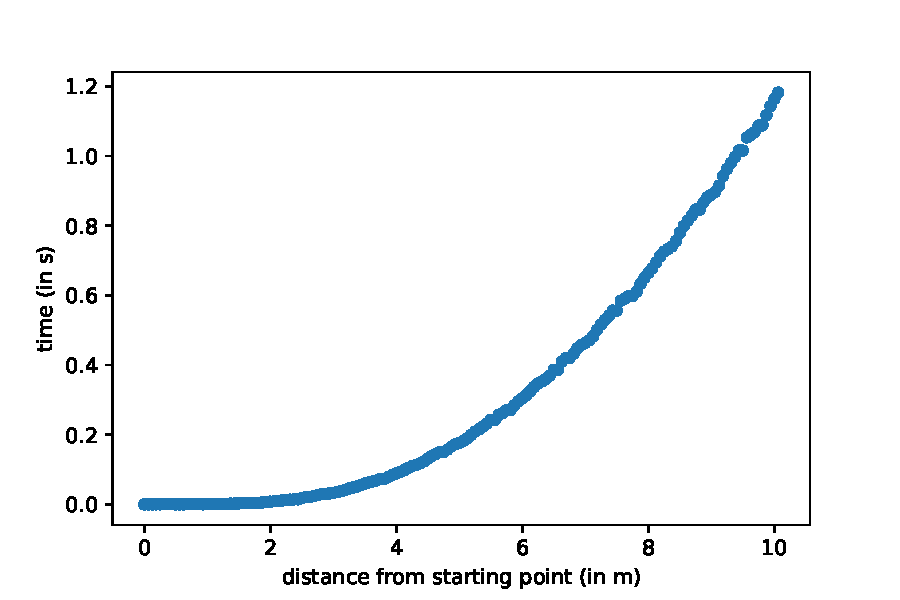
\includegraphics{figures/out-20-1_5-1.pdf}
    \caption{Plot of the distance (in $m$) from the starting point as the robot starts it's gait.}
    \label{fig:trajectory_1}
\end{figure}


\begin{figure}
    \centering
    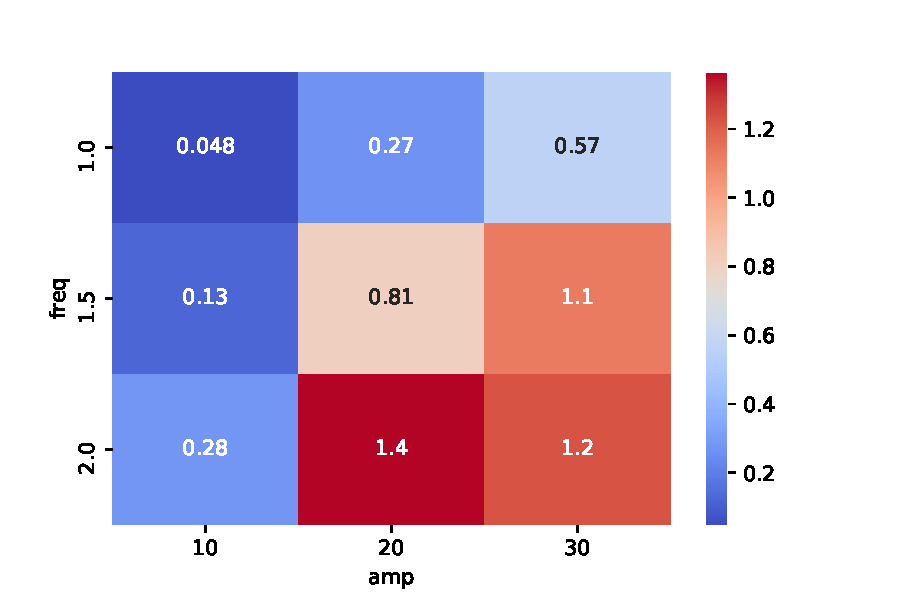
\includegraphics{figures/heatmap_speed.pdf}
    \caption{Heatmap representation of the speed (in $km/h$) as a function of oscillation frequency (in $Hz$) and amplitude (in degrees).}
    \label{fig:heatmap_speed}
\end{figure}

\textit{TODO : Point 7.2 (influence of frequency)}

\subsection{Optimizing the position controller}

\printbibliography %Prints bibliography

\end{document}
